\section{Problem 5: Cyclomatic Number}

\subsection{Calculating the Cyclomatic Number (Cyclomatic Complexity)}

To implement METRICSTICS, the object-oriented paradigm was used. There are 4 classes that were defined, with each assuming responsibility for specific functionalities: 
\begin{enumerate}
    \item \textbf{main.py}: involves the handling of the GUI functionalities
    \item \textbf{calculator.py}: descriptive statistics calculation functions
    \item \textbf{csv\_processor.py}: csv processing and functions
    \item \textbf{data\_validator.py}: functions to transform and validate data input for descriptive statistics calculation
\end{enumerate}

To obtain the cyclomatic complexity for each class, a tool called Radon was used. Radon is a Python tool that computes various code metrics, including cyclomatic complexity, which is a quantitative measure of code paths and a predictor of its maintainability. Utilizing Radon, we analyzed the METRICSTICS system to assess its complexity and infer the quality of the codebase. This report presents the cyclomatic complexity for each module and discusses the implications of these metrics on the system's overall maintainability and robustness. The following sections detail the complexity scores and provide a qualitative interpretation relative to standard thresholds.

\begin{enumerate}
\item \textbf{Cyclomatic Complexity for main.py}
    
\begin{figure}[!htb]
    \begin{center}
    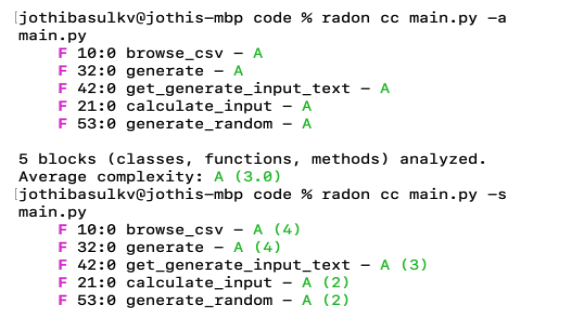
\includegraphics[width=10cm]{images/cc_main.png} % 
    \end{center}
    \caption{Cyclomatic Complexity for main.py}
\end{figure}

Average Cyclomatic Complexity: A (3.0)\\

\pagebreak
\item \textbf{Cyclomatic Complexity for calculator.py}

\begin{figure}[!htb]
    \centering
    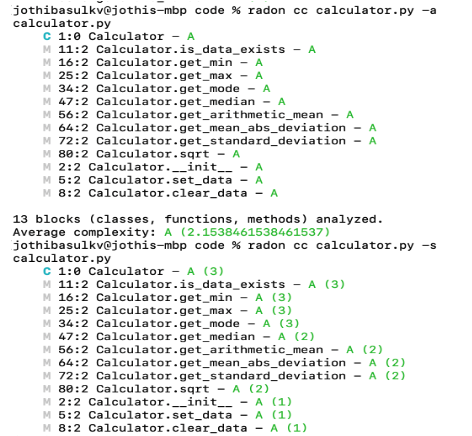
\includegraphics[width=10cm]{images/cc_calculator.png}
    \caption{Cyclomatic Complexity for calculator.py}
\end{figure}

Average Cyclomatic Complexity:  A (2.1538461538461537)\\

\item \textbf{Cyclomatic Complexity for csv\_processor.py}

\begin{figure}[!htb]
    \centering
    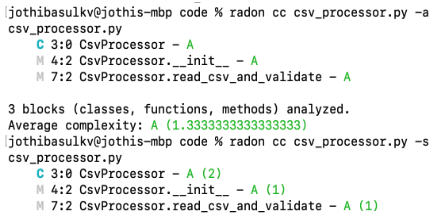
\includegraphics[width=10cm]{images/cc_csvprocessor.png}
    \caption{Cyclomatic Complexity for csv\_processor.py}
\end{figure}

Average Cyclomatic Complexity:  A (1.3333333333333333)\\

\pagebreak

\item \textbf{Cyclomatic Complexity for data\_validator.py}

\begin{figure}[!htb]
    \centering
    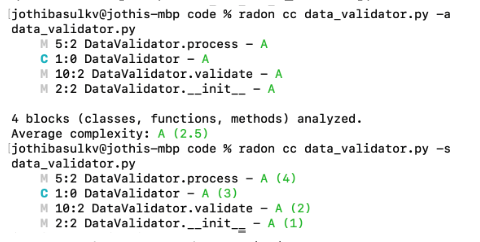
\includegraphics[width=10cm]{images/cc_datavalidator.png}
    \caption{Cyclomatic Complexity for data\_validator.py}
\end{figure}

Average Cyclomatic Complexity: A (2.5)
\end{enumerate}

\subsection{Qualitative Conclusions}

\begin{enumerate}
\item \textbf{Qualitative Conclusions for main.py}\\

\begin{enumerate}
    \item The functions \texttt{browse\_csv} and generate have the highest complexity scores of 4, which indicates that they have multiple paths for execution but remain within a reasonable range for understanding and maintenance.
    \item The \texttt{get\_generate\_input\_text} function has a slightly lower complexity score of 3, suggesting that it is simpler than the aforementioned functions, likely due to fewer conditional paths. 
    \item The \texttt{calculate\_input} and \texttt{generate\_random} functions have the lowest complexity scores of 2, which are indicative of straightforward, linear execution paths with minimal branching.
\end{enumerate}

\item \textbf{Qualitative Conclusions for calculator.py}\\

\begin{enumerate}
    \item The methods generally have low complexity scores (1 to 3), indicating that each method is likely doing one specific task with a clear and straightforward logic flow. 
    \item The uniformity of scores (mostly 3s and 2s) suggests consistent coding practices and potentially similar levels of abstraction across different methods.
    \item An average complexity score of slightly over 2 suggests that the \texttt{calculator.py} module is well within the range of good maintainability and should be straightforward to test.
    \item Such a low average score is a positive indicator of code quality, implying that there are few conditional branches within each method, which aligns with best practices in writing clear and concise code.
\end{enumerate}

\item \textbf{Qualitative Conclusions for csv\_processor.py}\\

\begin{enumerate}
    \item All methods in the \texttt{csv\_processor.py} module have low complexity scores, with the CsvProcessor class itself scoring a 2 and the methods \texttt{\_\_init\_\_} and \texttt{read\_csv\_and\_validate} both scoring a 1. 
    \item This indicates that the methods have a linear flow with minimal branching, which translates to a straightforward logic that is easy to follow and maintain.
    \item The average complexity of approximately 1.33 suggests that the module is very well-designed, with simplicity at its core. 
    \item The module's low complexity is indicative of a high-quality design that should facilitate easy testing and low risk of defects.
\end{enumerate}

\item \textbf{Qualitative Conclusions for data\_validator.py}\\

\begin{enumerate}
    \item \texttt{DataValidator} (the class itself) has a complexity of 3, suggesting that the class as a whole has some conditional logic but is not overly complex. 
    \item The \texttt{\_\_init\_\_} function has the lowest complexity, which is expected as constructors typically have a clear and single path of execution.
    \item The function \texttt{process} has the highest complexity with a score of 4, which might indicate multiple paths or decision points within the method, yet it remains at an acceptable level of complexity. 
    \item The \texttt{validate} function has a complexity of 2, which is indicative of a straightforward method with one or two decision points or loops. 
\end{enumerate}

\end{enumerate}

\pagebreak